% Options for packages loaded elsewhere
\PassOptionsToPackage{unicode}{hyperref}
\PassOptionsToPackage{hyphens}{url}
\PassOptionsToPackage{dvipsnames,svgnames,x11names}{xcolor}
%
\documentclass[
  letterpaper,
  DIV=11,
  numbers=noendperiod]{scrartcl}

\usepackage{amsmath,amssymb}
\usepackage{iftex}
\ifPDFTeX
  \usepackage[T1]{fontenc}
  \usepackage[utf8]{inputenc}
  \usepackage{textcomp} % provide euro and other symbols
\else % if luatex or xetex
  \usepackage{unicode-math}
  \defaultfontfeatures{Scale=MatchLowercase}
  \defaultfontfeatures[\rmfamily]{Ligatures=TeX,Scale=1}
\fi
\usepackage{lmodern}
\ifPDFTeX\else  
    % xetex/luatex font selection
\fi
% Use upquote if available, for straight quotes in verbatim environments
\IfFileExists{upquote.sty}{\usepackage{upquote}}{}
\IfFileExists{microtype.sty}{% use microtype if available
  \usepackage[]{microtype}
  \UseMicrotypeSet[protrusion]{basicmath} % disable protrusion for tt fonts
}{}
\makeatletter
\@ifundefined{KOMAClassName}{% if non-KOMA class
  \IfFileExists{parskip.sty}{%
    \usepackage{parskip}
  }{% else
    \setlength{\parindent}{0pt}
    \setlength{\parskip}{6pt plus 2pt minus 1pt}}
}{% if KOMA class
  \KOMAoptions{parskip=half}}
\makeatother
\usepackage{xcolor}
\setlength{\emergencystretch}{3em} % prevent overfull lines
\setcounter{secnumdepth}{-\maxdimen} % remove section numbering
% Make \paragraph and \subparagraph free-standing
\makeatletter
\ifx\paragraph\undefined\else
  \let\oldparagraph\paragraph
  \renewcommand{\paragraph}{
    \@ifstar
      \xxxParagraphStar
      \xxxParagraphNoStar
  }
  \newcommand{\xxxParagraphStar}[1]{\oldparagraph*{#1}\mbox{}}
  \newcommand{\xxxParagraphNoStar}[1]{\oldparagraph{#1}\mbox{}}
\fi
\ifx\subparagraph\undefined\else
  \let\oldsubparagraph\subparagraph
  \renewcommand{\subparagraph}{
    \@ifstar
      \xxxSubParagraphStar
      \xxxSubParagraphNoStar
  }
  \newcommand{\xxxSubParagraphStar}[1]{\oldsubparagraph*{#1}\mbox{}}
  \newcommand{\xxxSubParagraphNoStar}[1]{\oldsubparagraph{#1}\mbox{}}
\fi
\makeatother


\providecommand{\tightlist}{%
  \setlength{\itemsep}{0pt}\setlength{\parskip}{0pt}}\usepackage{longtable,booktabs,array}
\usepackage{calc} % for calculating minipage widths
% Correct order of tables after \paragraph or \subparagraph
\usepackage{etoolbox}
\makeatletter
\patchcmd\longtable{\par}{\if@noskipsec\mbox{}\fi\par}{}{}
\makeatother
% Allow footnotes in longtable head/foot
\IfFileExists{footnotehyper.sty}{\usepackage{footnotehyper}}{\usepackage{footnote}}
\makesavenoteenv{longtable}
\usepackage{graphicx}
\makeatletter
\newsavebox\pandoc@box
\newcommand*\pandocbounded[1]{% scales image to fit in text height/width
  \sbox\pandoc@box{#1}%
  \Gscale@div\@tempa{\textheight}{\dimexpr\ht\pandoc@box+\dp\pandoc@box\relax}%
  \Gscale@div\@tempb{\linewidth}{\wd\pandoc@box}%
  \ifdim\@tempb\p@<\@tempa\p@\let\@tempa\@tempb\fi% select the smaller of both
  \ifdim\@tempa\p@<\p@\scalebox{\@tempa}{\usebox\pandoc@box}%
  \else\usebox{\pandoc@box}%
  \fi%
}
% Set default figure placement to htbp
\def\fps@figure{htbp}
\makeatother

\KOMAoption{captions}{tableheading}
\makeatletter
\@ifpackageloaded{caption}{}{\usepackage{caption}}
\AtBeginDocument{%
\ifdefined\contentsname
  \renewcommand*\contentsname{Table of contents}
\else
  \newcommand\contentsname{Table of contents}
\fi
\ifdefined\listfigurename
  \renewcommand*\listfigurename{List of Figures}
\else
  \newcommand\listfigurename{List of Figures}
\fi
\ifdefined\listtablename
  \renewcommand*\listtablename{List of Tables}
\else
  \newcommand\listtablename{List of Tables}
\fi
\ifdefined\figurename
  \renewcommand*\figurename{Figure}
\else
  \newcommand\figurename{Figure}
\fi
\ifdefined\tablename
  \renewcommand*\tablename{Table}
\else
  \newcommand\tablename{Table}
\fi
}
\@ifpackageloaded{float}{}{\usepackage{float}}
\floatstyle{ruled}
\@ifundefined{c@chapter}{\newfloat{codelisting}{h}{lop}}{\newfloat{codelisting}{h}{lop}[chapter]}
\floatname{codelisting}{Listing}
\newcommand*\listoflistings{\listof{codelisting}{List of Listings}}
\makeatother
\makeatletter
\makeatother
\makeatletter
\@ifpackageloaded{caption}{}{\usepackage{caption}}
\@ifpackageloaded{subcaption}{}{\usepackage{subcaption}}
\makeatother

\usepackage{bookmark}

\IfFileExists{xurl.sty}{\usepackage{xurl}}{} % add URL line breaks if available
\urlstyle{same} % disable monospaced font for URLs
\hypersetup{
  pdftitle={Assignment 1},
  pdfauthor={Kyle Bradbury},
  colorlinks=true,
  linkcolor={blue},
  filecolor={Maroon},
  citecolor={Blue},
  urlcolor={Blue},
  pdfcreator={LaTeX via pandoc}}


\title{Assignment 1}
\usepackage{etoolbox}
\makeatletter
\providecommand{\subtitle}[1]{% add subtitle to \maketitle
  \apptocmd{\@title}{\par {\large #1 \par}}{}{}
}
\makeatother
\subtitle{Probability, Linear Algebra, and Computational Programming}
\author{Kyle Bradbury}
\date{2024-12-11}

\begin{document}
\maketitle

\renewcommand*\contentsname{Table of contents}
{
\hypersetup{linkcolor=}
\setcounter{tocdepth}{1}
\tableofcontents
}

\subsection{Instructions}\label{instructions}

\emph{Instructions for all assignments can be found
\href{https://kylebradbury.github.io/ids705/notebooks/assignment_instructions.html}{here}.
Note: this assignment falls under collaboration Mode 2: Individual
Assignment -- Collaboration Permitted. Please refer to the syllabus for
additional information. Please be sure to list the names of any students
that you worked with on this assignment. Total points in the assignment
add up to 90; an additional 10 points are allocated to professionalism
and presentation quality.}

Note: you may either write out equations by hand or using markdown and
\href{https://tobi.oetiker.ch/lshort/lshort.pdf}{LaTeX} (LaTeX is
recommended). Either way, I recommend that you complete the work on
paper before typing up the final version if you choose to use LaTeX. If
you hand-write your math, please digitize them (scan them in or take a
picture) and place them in the proper order for of the document for your
final PDF. Either way, show your math including any intermediate steps
necessary to understand the logic of your solution. If we are not able
to interpret your meaning (or understand your writing), no credit will
be given.

\subsection{Learning Objectives}\label{learning-objectives}

The purpose of this assignment is to provide a refresher on fundamental
concepts that we will use throughout this course and provide an
opportunity to develop skills in any of the related skills that may be
unfamiliar to you. Through the course of completing this assignment, you
will\ldots{}

\begin{itemize}
\tightlist
\item
  Refresh you knowledge of probability theory including properties of
  random variables, probability density functions, cumulative
  distribution functions, and key statistics such as mean and variance.
\item
  Revisit common linear algebra and matrix operations and concepts such
  as matrix multiplication, inner and outer products, inverses, the
  Hadamard (element-wise) product, eigenvalues and eigenvectors,
  orthogonality, and symmetry.
\item
  Practice numerical programming, core to machine learning, by applying
  it to scenarios of probabilistic modeling, linear algebra
  computations, loading and plotting data, and querying the data to
  answer relevant questions.
\item
  Apply your skills altogether through an exploratory data analysis to
  practice data cleaning, data manipulation, interpretation, and
  communication.
\end{itemize}

We will build on these concepts throughout the course, so use this
assignment as a catalyst to deepen your knowledge and seek help with
anything unfamiliar.

For references on the topics in this assignment, please check out the
\href{../resources.qmd\#}{resources} page on the course website for
online materials such as books and courses to support your learning.

\emph{Note: don't worry if you don't understand everything in the
references above - some of these books dive into significant minutia of
each of these topics.}

\newpage{}

\subsection{Exercise 1 - Probabilistic
Reasoning}\label{exercise-1---probabilistic-reasoning}

\textbf{1.1. Probabilistic Reasoning I.} You are handed three fair dice
and roll them sequentially. What's the probability of the sum of the
dice is 10 after you'be rolled the first die and it shows a 1?

\textbf{1.2. Probabilistic Computation I.} Simulate the scenario in 1.1
by creating 1 million synthetic rolls of the three dice. Determine what
fraction of outcomes that had a ``1'' for the first die also had a sum
of 10 across the three die.

\textbf{1.3. Probabilistic Reasoning II.} A test for a rare disease has
a 95\% chance of detecting the disease if a person has it (true positive
rate) and a 3\% chance of wrongly detecting it if a person does
\textbf{not} have it (false positive rate). If 1 in 1,000 people
\emph{actually} have the disease, what is the probability that a
randomly chosen person who tests positive actually has the disease?

\textbf{1.4. Discrete Probability Theory.} A discrete random variable
\(X\) is distributed as follows (probability mass function):

\(P(X = x) = \begin{cases}
                0.2 & x = -1 \\
                0.5 & x = 0 \\
                0.3 & x = 1
            \end{cases}\)

What is the expected value, \(E_X[X]\) and variance, \(Var_X(X)\) of the
random variable \(X\)?

\newpage{}

\subsection{Exercise 2 - Probability Distributions and
Modeling}\label{exercise-2---probability-distributions-and-modeling}

You've been asked to create a model of wait time for customers at
Olivander's Wand Shop. While they strive for the perfect match, there is
some cleanup between customers that has been keeping wait times high.
They're open 8 hours a day and the maximum wait time is 8 hours (we
won't assume it's possible not to be seen, assuming you're willing to
wait). Define the continuous random variable
\(X = \{\text{wait time for service as a fraction of 8 hours}\}\) . This
means that \(x=1\) represents a full day's wait, or 8 hours, \(x=0.5\)
represents half a day wait or 4 hours. Additionally, the valid values of
\(X\) are between 0 and 1 (\(0\leq x \leq 1\)).

We'll begin by analyzing some data of past visits to the shop to
understand the customer wait time experience through our data (2.1-2.2).
Then, we'll select a model we hypothesize might fit our situation well
and evaluate its properties like mean and variance (2.3-2.7). We'll also
evaluate the quality of the fit of the model as compare to our data
(2.8-2.11). Lastly, we'll explore how this approach can be used to
generate insights (2.12).

\subsubsection{Reviewing our wait time
data}\label{reviewing-our-wait-time-data}

\textbf{2.1. Load and plot a histogram of your wait time data.} The file
is \texttt{wait\_times.csv} in the \texttt{data/} folder. I recommend
using the simple \texttt{np.loadtxt()} function to accomplish this so
you can quickly load it in as a numpy array. Remember, the value 1
represents a full 8 hour work day so you should see your data are all in
the range of \([0,1]\). Please use 10 bins and limit the bin edges to
the range \([0,1]\) (no values should be plotted outside that range).

\textbf{2.2. Mean, variance, and standard deviation of the data.}
Compute the mean, variance, and standard deviation of the wait time
data. Report the mean and standard deviation in both the original units
(in \([0,1]\)) and in hours (the variance is unitless).

\subsubsection{Creating a model for the wait time
distribution}\label{creating-a-model-for-the-wait-time-distribution}

Take a moment to review the distribution of the data. The most common
distribution is normal, but this doesn't seem normally distributed.
Neither does it look uniform. The shape actually looks like it may be
exponentially distributed, but truncated at 1. It's not uncommon to have
this type of shape in a wait time model, but this introduces a challenge
since we can't just use the standard exponential distribution since an
exponential distribution is defined on a domain from 0 to infinity, but
our data is defined between 0 and 1. Let's create a customized
distribution as a model for our data and see how well it represents the
key statistics of our data.

In this section, please note the list of equations and identities at the
end of this document as they may be useful for several questions.

\textbf{2.3. Probability Density Functions (PDFs).} Compute the value of
\(\alpha\) that makes \(f_X(x)\) a valid probability density function:

\(f_X(x) = \begin{cases}
                \alpha e^{-x}  & 0 \leq x \leq 1 \\
                0           & \text{else}
            \end{cases}\)

Provide this value exactly (with no approximation) and also provide and
approximate decimal value with a precision to three decimal places.

\textbf{2.4. Cumulative Distribution Functions (CDFs).} Compute the
cumulative distribution function (CDF) of \(X\), \(F_X(x)\), where
\(F_X(x)=P(X<x)\) (here, \(P(\cdot)\) represents the probability of the
event within the brackets). Be sure to indicate the value of the CDF for
\textbf{\emph{all}} values of \(x\in(-\infty,\infty)\). Express your CDF
using the variable \(\alpha\) to provide the precise CDF.

\textbf{2.5. Expected Value.} Compute the expected value of \(X\),
\(E_X[X]\). Provide this value exactly (no approximations and only in
terms of \(e\) and \(\alpha\)) and provide a numerical approximation of
the variance to 3 decimal places. Also provide the approximate number of
hours waiting (to 3 decimal places).

\textbf{2.6. Variance and Standard Deviation.} Compute the variance of
\(X\), \(Var(X)\) approximately to 3 significant figures, meaning 3
digits without leading zeros (e.g.~12.3, 0.123, 0.00123, all have 3
significant figures). Using the variance, calculate the standard
deviation and express this standard deviation in both the original units
and units of hours.

\textbf{2.7. Plotting your functions.} Create functions to implement
your PDF, \(f_X(x)\), and CDF, \(F_X(x)\), for all possible values of
\(x\). Using these functions, plot the PDF and CDF on the inverval
\(-0.5 \leq x \leq 1.5\).

\subsubsection{Evaluating the quality of the
model}\label{evaluating-the-quality-of-the-model}

\textbf{2.8. Compare the empirical CDF to the modeled CDF.} Plot both of
these on the interval \(0 \leq x \leq 1\). For the empirical CDF of the
data from \texttt{wait\_times.csv}, you can plot the empirical CDF by
sorting the data in ascending order, your \(x\) values, and assigning
the \(y\) value as the cumulative fraction of samples that are smaller
than or equal to each \(x\) value.

\textbf{2.9. Calculate the inverse CDF to enable you to generate
synthetic data.} Create a numerical simulation of this process. Doing
this for a custom PDF is easier than you may think. We typically have
access to uniformly distributed samples (through
\texttt{np.random.rand}), and we can transform these uniform samples
into any distribution we wish. To do this, we can input uniform variates
through the \emph{inverse} of the CDF. If \(U\) is a uniformly
distributed random variable and \(F_X(x)\) is the CDF of the
distribution we're looking to model, then \(F_X^{-1}(U)\) will be
distributed in the same way as \(X\), as shown below in Figure 1.

\begin{figure}[H]

{\centering \pandocbounded{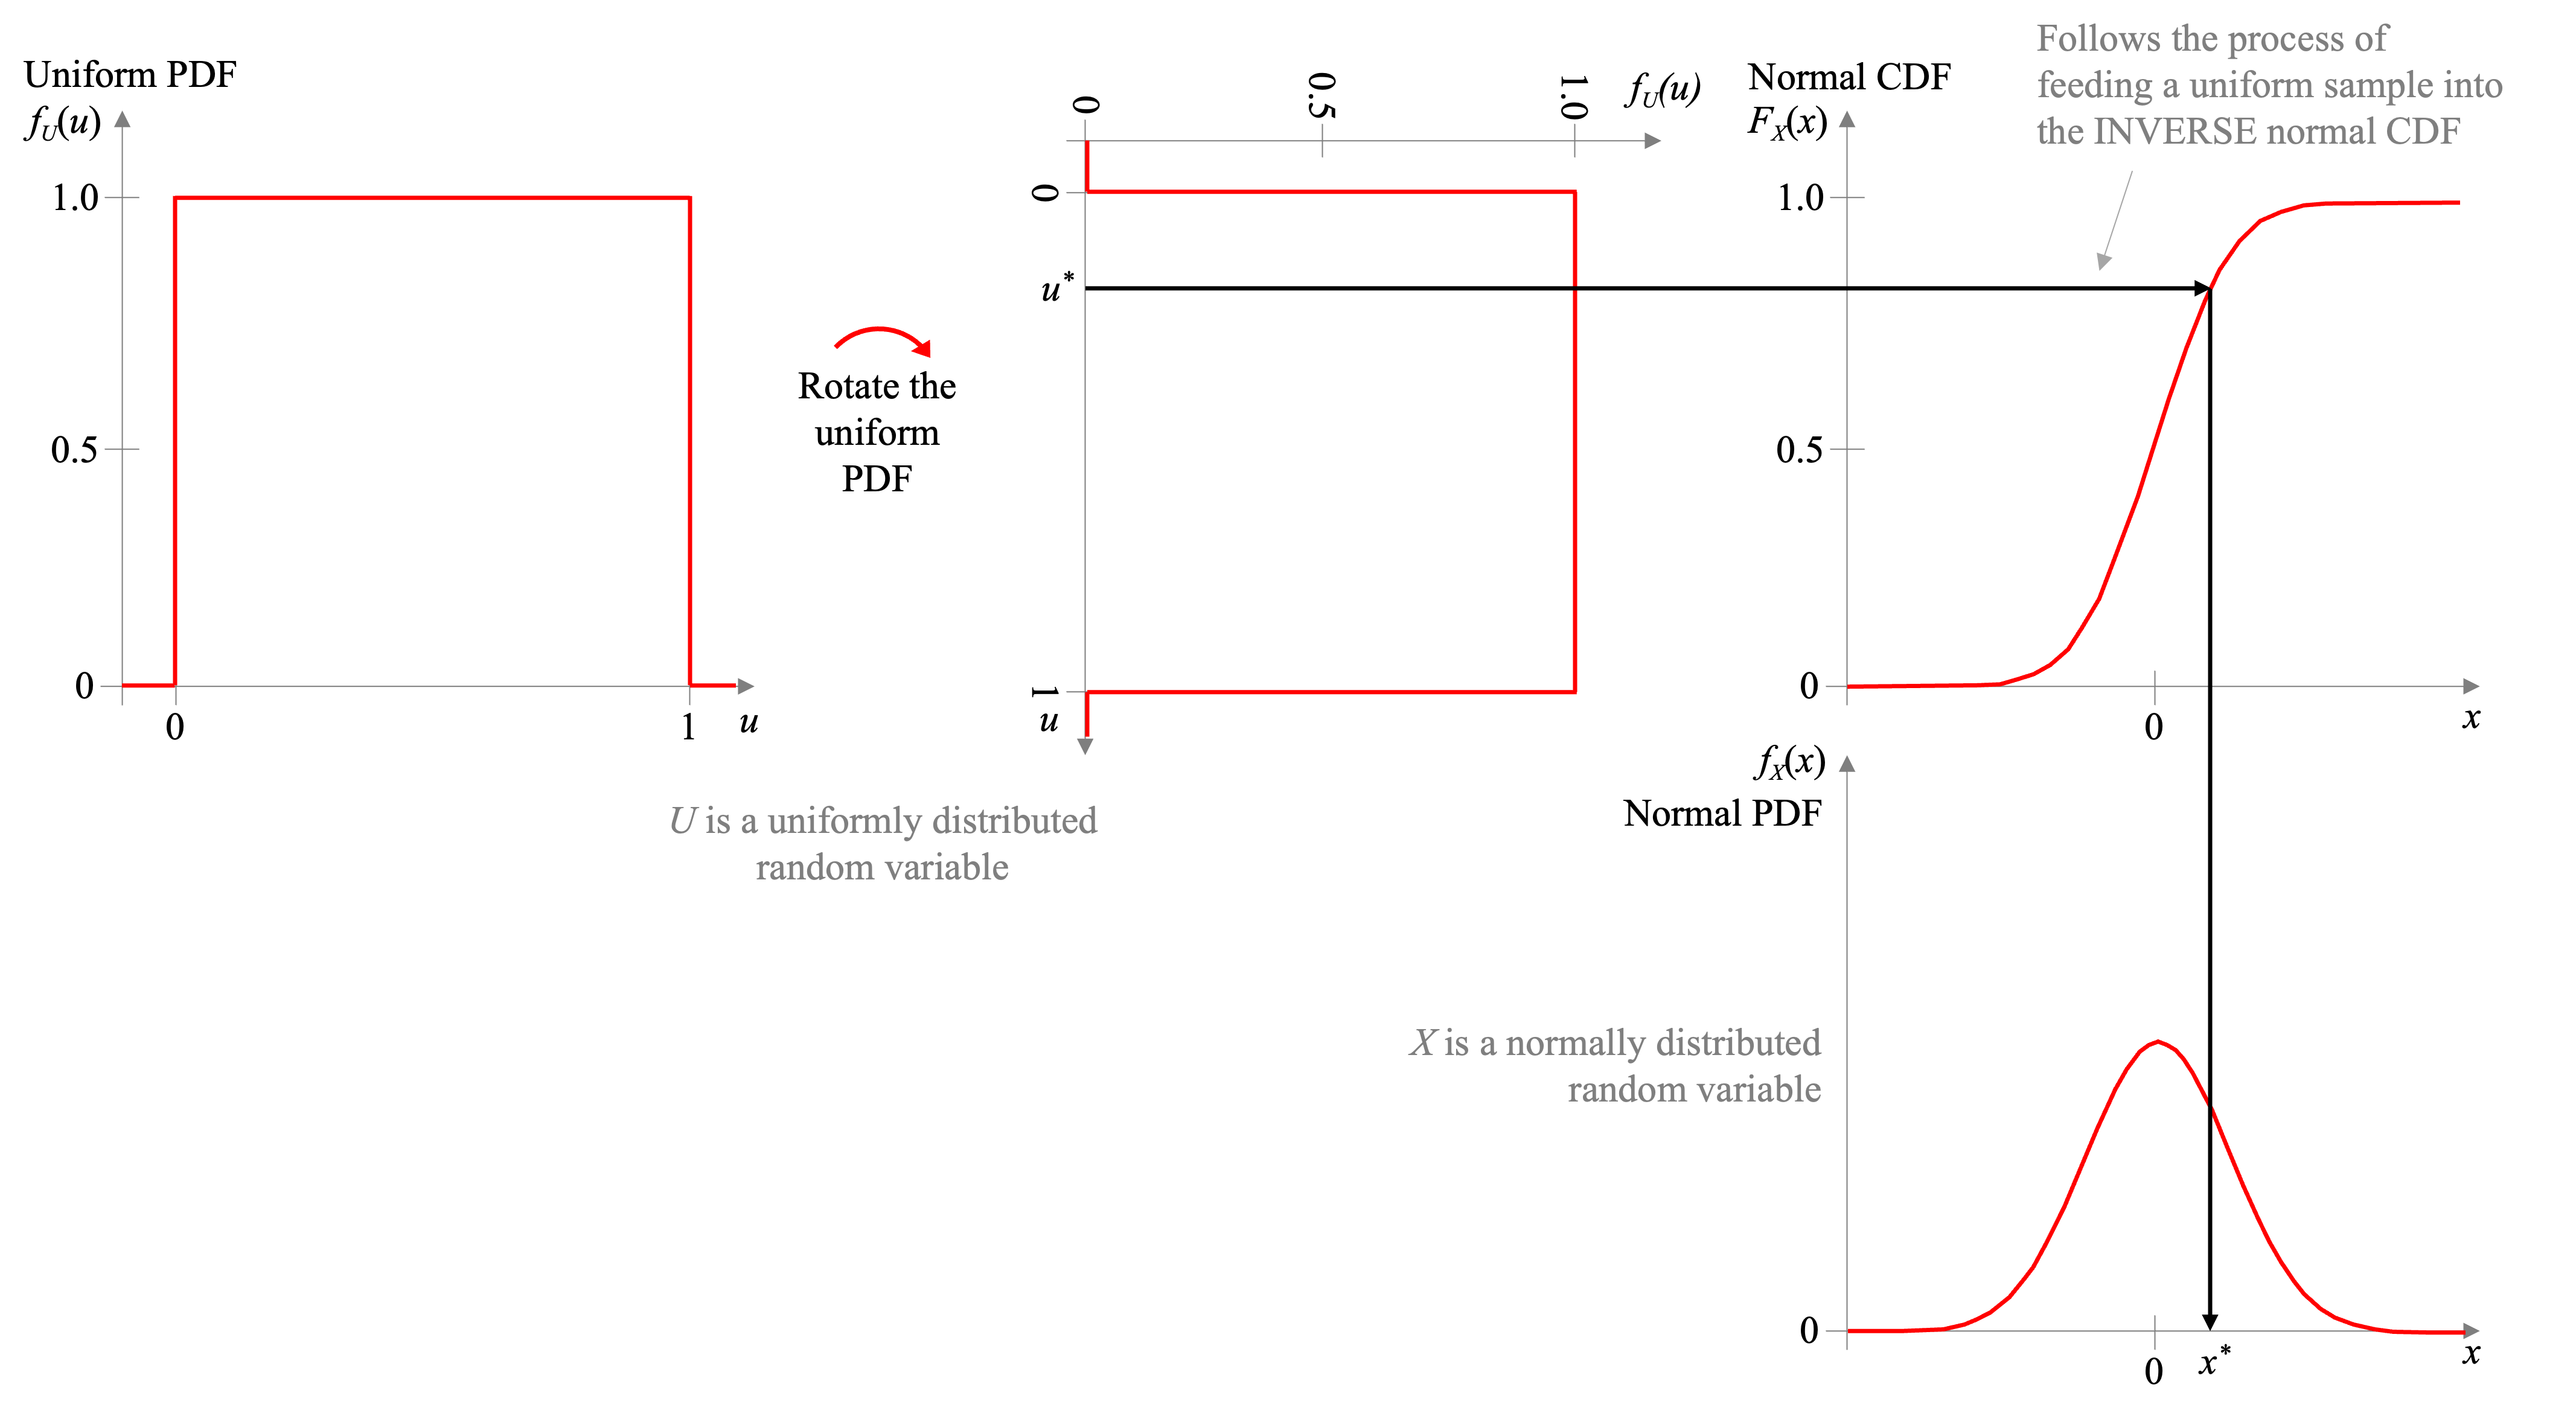
\includegraphics[keepaspectratio]{img/copula.png}}

}

\caption{Synthetic Data Generation}

\end{figure}%

\emph{Figure 1. Demonstrating the process of transforming a uniformly
distributed random variable into almost any distribution (here we
transform into a normal). Here we show the transformation a sample,
\(u^{\ast}\), from a uniform distribution to a sample, \(x^{\ast}\) from
a normal distribution by applying the inverse of the CDF of \(X\) to
\(u^{\ast}\), that is \(x^{\ast} = F_X^{-1}(u^{\ast})\).}

Calculate the inverse of the CDF, \(F_X^{-1}(y)\) (We use the variable
\(y\) as the input into this function to denote that we're inputting the
``output'' of the CDF into this inverse CDF).

\textbf{2.10. Generate synthetic data using the inverse CDF by
transforming uniform samples.} Once you have your inverse CDF, code it
up and use it to create synthetic samples from the last step. To do so,
first generate 10,000 samples from the uniform distribution and then
feed those uniform variates through the inverse CDF to generate
synthetic variates from our wait time model. Using those samples,
compute the mean and standard deviation. Present the mean and standard
deviation in a table comparing (a) the empirical values computed from
\texttt{wait\_times.csv}, your theoretical model values calculated
earlier, and your computed values calculated from your synthetic model.
How do they compare?

\textbf{2.11. Run a statistical test to evaluate the goodness of fit of
your model to the empirical data from \texttt{wait\_times.csv}.} To
evaluate the goodness of fit of the model to the data, one tool is the
Kolmogorov--Smirnov test, or simply the KS test. The two-sample version
of this test evaluates the maximum distance between two CDFs, each
calculated from samples of data. In this case, the null hypothesis
states that the samples are drawn from the same distribution. We can
conclude that the sample data are well-represented by the reference
distribution if we do NOT reject the null hypothesis. If we test at the
5\% significant level, then we can conclude that data come from the same
distribution if the p-value is greater than 0.05 (we fail to reject the
null hypothesis).

Compare the sample of data from \texttt{wait\_times.csv} to the
synthetic sample from the model distribution and run the KS test. Also
compare the sample data to the uniform distributed data you generated
before transforming it into the synthetic samples. For the test use
\href{https://docs.scipy.org/doc/scipy/reference/generated/scipy.stats.kstest.html}{\texttt{scipy.stats.kstest}}.

\subsubsection{Using the model to understand wait
times}\label{using-the-model-to-understand-wait-times}

\textbf{2.12. Computing probabilities.} Having a way of generating
synthetic data can allow us to easily compute probabilities. Compute the
probabilities of the following events using the \emph{synthetic data
samples} that you generated.

\begin{enumerate}
\def\labelenumi{\arabic{enumi}.}
\tightlist
\item
  Wait time is more than 6 hours
\item
  Wait time is less than 1 hour
\item
  Wait time is less than one hour given the client has already been
  waiting for 3 hours
\item
  Wait time is between 3 and 5 hours
\item
  What is the 90th percentile of wait times?
\item
  What is the 99th percentile of wait times?
\end{enumerate}

\newpage{}

\subsection{Exercise 3 - Linear Algebra Operations and
Theory}\label{exercise-3---linear-algebra-operations-and-theory}

\textbf{3.1. Matrix manipulations and multiplication}. Machine learning
involves working with many matrices and understanding what their
products represent, so this exercise will provide you with the
opportunity to practice those skills.

Let \(\mathbf{A} =  \begin{bmatrix}
1 & 2 \\
3 & 4
\end{bmatrix}\), \(\mathbf{b} =  \begin{bmatrix}
-1  \\
1
\end{bmatrix}\), \(\mathbf{c} =  \begin{bmatrix}
1  \\
2
\end{bmatrix}\)

Compute the following \textbf{by hand} or indicate that it cannot be
computed. For any cases where an operation is invalid and cannot be
computed, explain why it is invalid.

\begin{enumerate}
\def\labelenumi{\arabic{enumi}.}
\tightlist
\item
  \(\mathbf{A}\mathbf{A}\)
\item
  \(\mathbf{A}\mathbf{A}^{\top}\)
\item
  \(\mathbf{A}\mathbf{b}\)
\item
  \(\mathbf{A}\mathbf{b}^{\top}\)
\item
  \(\mathbf{b}\mathbf{A}\)
\item
  \(\mathbf{b}^{\top}\mathbf{A}\)
\item
  \(\mathbf{b}\mathbf{b}\)
\item
  \(\mathbf{b}^{\top}\mathbf{b}\)
\item
  \(\mathbf{b}\mathbf{b}^{\top}\)
\item
  \(\mathbf{A}\circ\mathbf{A}\)
\item
  \(\mathbf{b}\circ\mathbf{c}\)
\item
  \(\mathbf{b}^{\top}\mathbf{b}^{\top}\)
\item
  \(\mathbf{b} + \mathbf{c}^{\top}\)
\item
  \(\mathbf{A}^{-1}\mathbf{b}\)
\item
  \(\mathbf{b}^{{\top}}\mathbf{A}\mathbf{b}\)
\item
  \(\mathbf{b}\mathbf{A}\mathbf{b}^{{\top}}\)
\end{enumerate}

\emph{Note: The element-wise (or Hadamard) product is the product of
each element in one matrix with the corresponding element in another
matrix, and is represented by the symbol ``\(\circ\)''.}

\textbf{3.2. Matrix manipulations and multiplication using Python}.
Repeat 3.1, but this time using Python. If you are using a vector, make
sure the dimensions of the vector match what you'd expect, for example,
matrix \(\mathbf{b}\) is a \([2 \times 1]\) vector. In NumPy, unless
you're specify, you'll like create a one-dimensional array of length 2
rather than a \([2 \times 1]\) vector if you don't specify - be careful
of this potential pitfall. Refer to NumPy's tools for handling matrices.
There may be circumstances when Python \textbf{will} produce an output,
but based on the dimensions of the matrices involved, the linear algebra
operation is not possible. \textbf{\emph{Note these cases and explain
why they occur}}. Please provide both the Python code AND the output of
that code showing your result. If the output is an error, comment out
the code and note that it cannot be computed.

Be sure to use the right operator for each operation: Matrix
multiplication: \texttt{@}; Element-wise multication: \texttt{*}. For
this exercise, \textbf{only} use one of those to operators for matrix or
vector multiplication.

\textbf{3.3. Vector Norms.} Norms are the effective lengths of vectors.
For example, the Euclidean norm, or \(L_2\) norm (denoted as
\(||\mathbf{\cdot}||_2\)), is the most common of several types of norms.
The \(L_2\) norm can be calculated for a vector
\[\mathbf{x} =  \begin{bmatrix} x_1 \\ x_2 \\ \vdots \\ x_n \end{bmatrix}\]
as follows:
\[||\mathbf{x}||_2 = \sqrt{\displaystyle \sum_{k=1}^n x_k^2} = \sqrt{\mathbf{x}^{\top}\mathbf{x}}\]

What is the \(L_2\) norm of vectors
\(\mathbf{d}_1 =  \begin{bmatrix} 2^{-1/2} \\ -2^{-1/2} \\ 0 \end{bmatrix}\)
and \(\mathbf{d}_2 = \begin{bmatrix} 0 \\ 0 \\ 1 \end{bmatrix}\)?

\textbf{3.4. Orthogonality and unit vectors.} Orthogonal vectors are
frequently used in machine learning in topics such as Principal
Components Analysis and feature engineering for creating decorrelated
features. Knowing what an orthogonal or orthonomal basis is for a space
is an important concept. Find all values of unit vectors,
\(\mathbf{d}_3\), that complete an orthonormal basis in a
three-dimensional Euclidean space along with the two vectors:
\(\mathbf{d}_1 =  \begin{bmatrix} 2^{-1/2} \\ -2^{-1/2} \\ 0 \end{bmatrix}\)
and \(\mathbf{d}_2 = \begin{bmatrix} 0 \\ 0 \\ 1 \end{bmatrix}\).

For review, vector \(\mathbf{x}_1\) is orthonormal to vector
\(\mathbf{x}_2\) if (a) \(\mathbf{x}_1\) is orthogonal to vector
\(\mathbf{x}_2\) AND \(\mathbf{x}_1\) is a unit vector. Orthogonal
vectors are perpendicular, which implies that their inner product is
zero. A unit vector is of length 1 (meaning its \(L_2\) norm is 1).

\textbf{3.5. Eigenvectors and eigenvalues}. Eigenvectors and eigenvalues
are useful for numerous machine learning algorithms, but the concepts
take time to solidly grasp. They are used extensively in machine
learning including in Principal Components Analysis (PCA) and clustering
algorithms. For an intuitive review of these concepts, explore this
\href{http://setosa.io/ev/eigenvectors-and-eigenvalues/}{interactive
website at Setosa.io}. Also, the series of linear algebra videos by
Grant Sanderson of 3Brown1Blue are excellent and can be viewed on
youtube
\href{https://www.youtube.com/playlist?list=PLZHQObOWTQDPD3MizzM2xVFitgF8hE_ab}{here}.
For these questions, numpy may once again be helpful.

\begin{enumerate}
\def\labelenumi{\arabic{enumi}.}
\tightlist
\item
  In Python, calculate the eigenvalues and corresponding eigenvectors of
  matrix \(\mathbf{B}=  \begin{bmatrix}
  1 & 2 & 3 \\
  2 & 4 & 5 \\
  3 & 5 & 6
  \end{bmatrix}\)
\item
  Choose one of the eigenvector/eigenvalue pairs, \(\mathbf{v}\) and
  \(\lambda\), and show that
  \(\mathbf{B} \mathbf{v} = \lambda \mathbf{v}\). This relationship
  extends to higher orders:
  \(\mathbf{B} \mathbf{B} \mathbf{v} = \lambda^2 \mathbf{v}\)
\item
  Show that the eigenvectors are orthogonal to one another (e.g.~their
  inner product is zero - just compute the inner product and show it is
  approximately 0). This is true for eigenvectors from real, symmetric
  matrices. In three dimensions or less, this means that the
  eigenvectors are perpendicular to each other. Typically we use the
  orthogonal basis of our standard x, y, and z, Cartesian coordinates,
  which allows us, if we combine them linearly, to represent any point
  in a 3D space. But any three orthogonal vectors can do the same. This
  property is used, for example, in PCA to identify the dimensions of
  greatest variation.
\end{enumerate}

\newpage{}

\subsection{Exercise 4 - Numerical Programming with
Data}\label{exercise-4---numerical-programming-with-data}

\textbf{Loading data and gathering insights from a real dataset.} In
data science, we often need to have a sense of the idiosyncrasies of the
data, how they relate to the questions we are trying to answer, and to
use that information to help us to determine what approach, such as
machine learning, we may need to apply to achieve our goal. This
exercise provides practice in exploring a dataset and answering question
that might arise from applications related to the data.

\textbf{Your objective}. For this dataset, your goal is to answer the
questions below about electricity generation in the United States.

\textbf{Data}. The data for this problem can be found in the
\texttt{data\textbackslash{}a1\textbackslash{}} subfolder in the
\texttt{assignments} folder on
\href{https://github.com/kylebradbury/ids705}{github}. The filename is
\texttt{egrid2016.xlsx}. This dataset is the Environmental Protection
Agency's (EPA)
\href{https://www.epa.gov/energy/emissions-generation-resource-integrated-database-egrid}{Emissions
\& Generation Resource Integrated Database (eGRID)} containing
information about all power plants in the United States, the amount of
generation they produce, what fuel they use, the location of the plant,
and many more quantities. We'll be using a subset of those data.

The fields we'll be using include:

\begin{longtable}[]{@{}ll@{}}
\toprule\noalign{}
field & description \\
\midrule\noalign{}
\endhead
\bottomrule\noalign{}
\endlastfoot
SEQPLT16 & eGRID2016 Plant file sequence number (the index) \\
PSTATABB & Plant state abbreviation \\
PNAME & Plant name \\
LAT & Plant latitude \\
LON & Plant longitude \\
PLPRMFL & Plant primary fuel \\
CAPFAC & Plant capacity factor \\
NAMEPCAP & Plant nameplate capacity (Megawatts MW) \\
PLNGENAN & Plant annual net generation (Megawatt-hours MWh) \\
PLCO2EQA & Plant annual CO2 equivalent emissions (tons) \\
\end{longtable}

For more details on the data, you can refer to the
\href{https://www.epa.gov/sites/default/files/2020-01/documents/egrid2018_technical_support_document.pdf}{eGrid
technical documents}. For example, you may want to review page 51 and
the section ``Plant Primary Fuel (PLPRMFL)'', which gives the full names
of the fuel types including WND for wind, NG for natural gas, BIT for
Bituminous coal, etc.

There also are a couple of ``gotchas'' to watch out for with this
dataset: - The headers are on the second row and you'll want to ignore
the first row (they're more detailed descriptions of the headers). - NaN
values represent blanks in the data. These will appear regularly in
real-world data, so getting experience working with these sorts of
missing values will be important.

Questions to answer:

\textbf{4.1.} Which power plant generated the most energy in 2016
(measured in MWh)?

\textbf{4.2.} Which power plant produced the most CO2 emissions
(measured in tons)?

\textbf{4.3.} What is the primary fuel of the plant with the most CO2
emissions?

\textbf{4.4.} What is the name of the northern-most power plant in the
United States?

\textbf{4.5.} What is the state where the northern-most power plant in
the United States is located?

\textbf{4.6.} Plot a bar plot showing the amount of energy produced by
each fuel type across all plants.

\textbf{4.7.} From the plot in (D), which fuel for generation produces
the most energy (MWh) in the United States?

\textbf{4.8.} Which state has the largest number of hydroelectric
plants? In this case, each power plant counts once so regardless of how
large the power plant is, we want to determine which state has the most
of them. Note the primary fuel for hydroelectric plants is listed as
water in the documentation.

\textbf{4.9.} Which state(s) has generated the most energy (MWh) using
coal? If there are more than one, list the state abbreviations in
alphabetical order, separated with commas (but no spaces). You may also
want to explore the documentation for the \texttt{isin()} method for
pandas. Note: in the eGrid documentation, there are multiple types of
coal listed; be sure to factor in each type of coal.

\textbf{4.10.} Which primary fuel produced the \emph{most} CO2 emissions
in the United States? We would like to compare natural gas, coal, oil,
and renewables but the current categories are much more specific than
that. As a first step, group the data as shown below, replacing the
existing labels with the replacements suggested. For example, BIT and
LIG should be replaced with COAL. - COAL = BIT, LIG, RC, SUB, WC - OIL =
DFO, JF, KER, RFO, WO - GAS = BFG, COG, LFG, NG, OG, PG, PRG - RENEW =
GEO, SUN, WAT, WDL, WDS, WND

You may want to create a function that does this replacement prior to
running your code. You can check whether or not it was successful by
verifying that each of the values that should be replaced has been
replaced - check that before moving on with the question.

You will want to use `PLCO2EQA' to answer this question as it's the
quantity of emissions each plant generates.

\newpage{}

\subsection{Appendix: Definitions and
identities}\label{appendix-definitions-and-identities}

The symbology in this assignment conforms to the following convention:

\begin{longtable}[]{@{}
  >{\raggedright\arraybackslash}p{(\linewidth - 4\tabcolsep) * \real{0.3636}}
  >{\raggedright\arraybackslash}p{(\linewidth - 4\tabcolsep) * \real{0.3182}}
  >{\raggedright\arraybackslash}p{(\linewidth - 4\tabcolsep) * \real{0.3182}}@{}}
\toprule\noalign{}
\begin{minipage}[b]{\linewidth}\raggedright
Symbol Example
\end{minipage} & \begin{minipage}[b]{\linewidth}\raggedright
Meaning
\end{minipage} & \begin{minipage}[b]{\linewidth}\raggedright
Possible variations
\end{minipage} \\
\midrule\noalign{}
\endhead
\bottomrule\noalign{}
\endlastfoot
\(X\) & A random variable & Upper case, non-bolded letter \\
\(\bar{X}\) & The complement of a random variable & Upper case,
non-bolded letter with bar \\
\(\mathbf{x}\) & Vector (\(N \times 1\)) & Lower case, bolded
letters/symbols \\
\(\mathbf{X}\) & Matrix (\(N \times M\)) & Upper case, bolded
letters/symbols \\
\(P(\cdot)\) & Probability of the event within the parenthesis &
Parenthesis may include one event or more events \\
\(A \cap B\) & Intersection of \(A\) and \(B\), that is the case of
events \(A\) and \(B\) occurring simultaneously & Two random variables
represented by upper case unbolded letters \\
\end{longtable}

Below is a list of potentially helpful identities and equations for
reference.

\begin{longtable}[]{@{}
  >{\raggedright\arraybackslash}p{(\linewidth - 2\tabcolsep) * \real{0.5333}}
  >{\raggedright\arraybackslash}p{(\linewidth - 2\tabcolsep) * \real{0.4667}}@{}}
\toprule\noalign{}
\begin{minipage}[b]{\linewidth}\raggedright
Identities and equations
\end{minipage} & \begin{minipage}[b]{\linewidth}\raggedright
Description
\end{minipage} \\
\midrule\noalign{}
\endhead
\bottomrule\noalign{}
\endlastfoot
\(E_X[X] = \displaystyle \int_{-\infty}^{\infty} x f_X(x) dx\) &
Expected value of continuous random variable \(X\) \\
\(Var_X(X) = E_X[X^2]-E_X[X]^2\) & Variance of random variable \(X\) \\
\(\sigma_X(X) = \sqrt{Var_X(X)}\) & Standard deviation of \(X\) as a
function of variance \\
\(\displaystyle P( X \vert Y)= \frac{P(X \cap Y)}{P(Y)}\) & Conditional
probability of event \(X\) given event \(Y\) has occurred \\
\(\displaystyle P(Y \vert X)= \frac{P(X \vert Y)P(Y)}{P(X)}\) & Bayes'
Rule \\
\(\displaystyle F_X(x) = \int_{-\infty}^{x} f_X(x) dx\) & CDF as a
function of PDF \\
\(\displaystyle f_X(x) = \frac{dF_X(x)}{dx}\) & PDF as a function of
CDF \\
\(P(X \leq x) = F_X(x)\) & Probabilistic definition of the CDF \\
\(P(a < X \leq b) = F_X(b) - F_X(a)\) & Probability the \(X\) lies
between \(a\) and \(b\) \\
\(P(A) + P(\bar{A}) = 1\) & The sum of the probability of an event and
its complement is 1 \\
\(\displaystyle P(Y) = P(Y \vert X)P(X) + P(Y  \vert \bar{X})P(\bar{X})\)
& Law of Total Probability \\
\(\displaystyle \int e^{-x} dx = -e^{-x}\) & Indefinite integral \\
\(\displaystyle \int x e^{-x} dx = -e^{-x}(x+1)\) & Indefinite
integral \\
\(\displaystyle \int x^2 e^{-x} dx = -e^{-x}(x^2+2x+2)\) & Indefinite
integral \\
\(\displaystyle \begin{bmatrix} a & b \\ c & d \end{bmatrix}^{-1} = \frac{1}{ad-cb} \begin{bmatrix} d & -b \\ -c & a \end{bmatrix}\)
& \(2 \times 2\) matrix inversion formula \\
\end{longtable}




\end{document}
